\section{Texturing}
Il concetto di \textbf{texture} è molto importante nella Grafica Computazionale \\
\begin{itemize}
    \item Texturing $\rightarrow$ modulare un attributo dei vertici per ottenere un effetto visivo
    \item Possibili attributi dei vertici: colore, normale, trasparenza, un parametro dell'equazione di illuminazione, ecc.
    \item L'attributo più immediato per trasmettere dettagli visivi alla superficie è il colore.
    \item La modulazione dell'attributo colore è chiamata texture mapping
\end{itemize}
Durante le operazioni sui frammenti è possibile accedere a una particolare RAM, chiamata \textit{texture RAM}, che contiene un insieme di texture.
Ogni texture è un array 1D, 2D o 3D di texel (\textbf{texel} = campione di texture, pixel = campione di immagine) dello stesso tipo di dati.
\subsection{Texels}
\begin{itemize}
    \item Un texel è un colore (componenti: R-G-B o R-G-B-A): la texture è una mappa dei colori
    \item Un texel rappresenta il componente alpha: la texture è una mappa alpha
    \item Un texel è una normale (componenti: X-Y-Z): la texture è una mappa delle normali
    \item Un texel è un coefficiente speculare: la texture è una mappa di brillantezza
\end{itemize}
\begin{figure}[H]
    \centering
    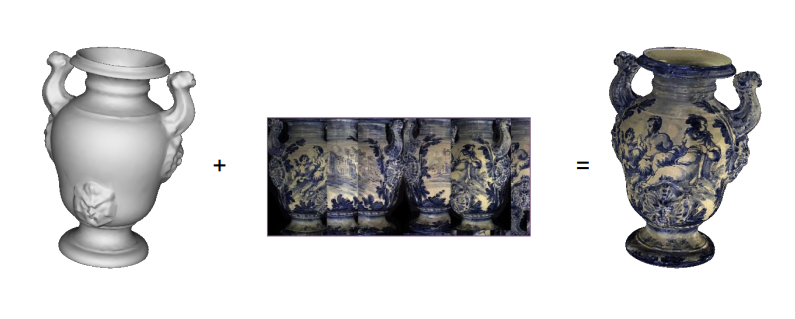
\includegraphics[width=0.5\textwidth]{images/Texturing.png} 
    \caption{Esempio di processo di texturing}
    \label{fig:immagine}
\end{figure}
Il texture space è anceh chiamato spazio uv, le coordinate nello spazio uv sono assegnate ad ogni vertice.
\begin{figure}[H]
    \centering
    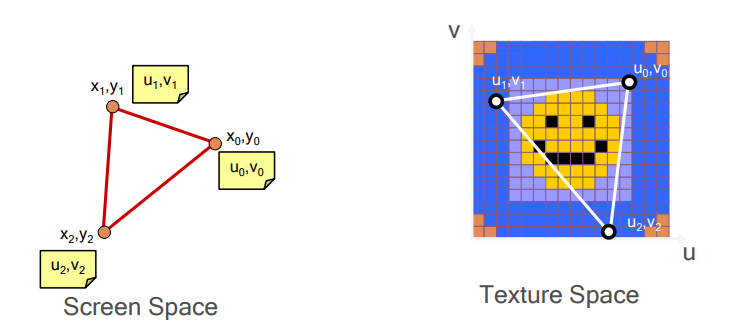
\includegraphics[width=0.5\textwidth]{images/TextMap.png} 
    \caption{Texturing mapping}
    \label{fig:immagine}
\end{figure}
Questo definisce un mapping tra i triangoli e le texture.
\subsection{Attribute Interpolation \& Coordinare Baricentriche}
Le coordinate baricentriche sono utilizzate
\begin{itemize}
    \item Cosa sono le coordinate baricentriche?
    \item Ricorda che un segmento può essere scritto come combinazione lineare di due punti:
    \item $ x=av_1 + bv_2 \\ a and b positive scalars with a + b = 1 \\ (=> 0 < a <= 1 and 0 <= b <= 1)$
    
\end{itemize}
\begin{figure}[H]
    \centering
    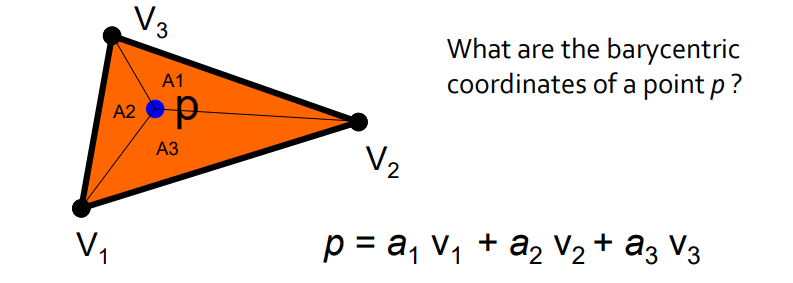
\includegraphics[width=0.5\textwidth]{images/Baric.png} 
    \caption{Barycentric Coordiantes}
    \label{fig:immagine}
\end{figure}
Un trinagolo di veritici $v_1,v_2,v_3 $ sono un insieme di punti tali che:\\ 
$x=a_1v_1+a_2v_2+a_3v_3 \\
\vspace{10pt} 
a_1,a_2,a_3 scalari positivi \\
\vspace{10pt} 
a_1+a_2+a_3=1 \\  $

L'interpolazione delle coordinate baricentriche non funziona quando le coordinate della texture sono interpolate a causa della proiezione prospettica. 
Funziona per altri attributi (ad esempio, per le normali).

\subsubsection{interpolazione delle coordinate della texture}
$p=c_0v_0+c_1v_1+c_2v_2$ \\
\vspace{10pt} 
\textbf{Attributi} di P: \\
\vspace{10pt} 
(senza la Perspective correction) \\
\vspace{10pt} 
$A_p=c_0A_0+c_1A_1+c_2A_2$ \\
\vspace{10pt} 
$B_p=c_0B_0+c_1B_1+c_2B_2$ \\
\vspace{10pt} 
$p=c_0v_0+c_1v_1+c_2v_2 $\\
\vspace{10pt} 
(con la Perspective correction) \\
$A_p=\frac{c_0\frac{A_0}{w_0}+c_1\frac{A_1}{w_1}+c_2\frac{A_2}{w_2}}{c_0\frac{1}{w_0}+c_1\frac{1}{w_1}+c_2\frac{1}{w_2}}
$
\begin{figure}[H]
    \centering
    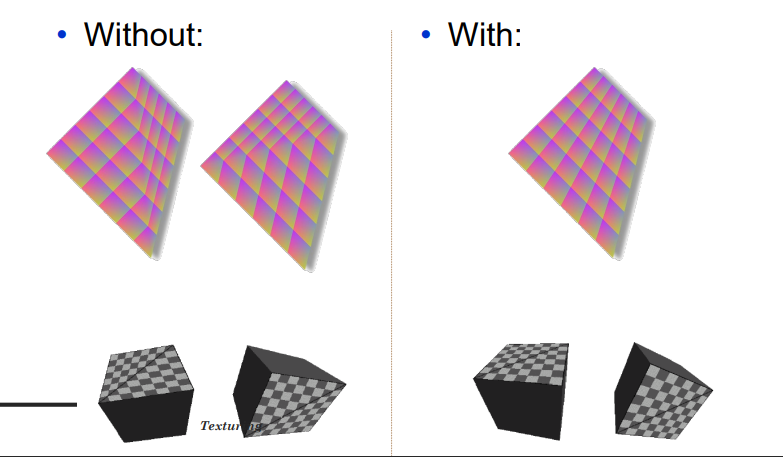
\includegraphics[width=0.5\textwidth]{images/PerspCorr.png} 
    \caption{Perspective Correction}
    \label{fig:immagine}
\end{figure}
Dalla RAM della CPU, la texture deve essere copiata nella RAM della texture per poter essere utilizzata.
L'inverso è possibile.
Entrambe le operazioni sono lente, quindi è importante progettare la tua applicazione grafica per ottimizzare i trasferimenti delle texture.
Come assegnare le coordinate della texture?
\begin{itemize}
    \item Calcolare le coordinate della texture al volo durante il rendering
    \item Precomputarle e memorizzarle nella mesh
    \item Spesso assegnate durante la fase di modellazione
\end{itemize}
Non esiste una soluzione ideale, dipende dall'applicazione.

\subsection{UV Mapping}

UV Mapping: il problema di assegnare le coordinate della texture a ciascun vertice della mesh come passaggio di pre-elaborazione.
Usiamo una funzione di proiezione per fare il mapping dalle corodinate (x,y,z) a quelle (u,v)
Planar projection(asse x): \\

$ (x,y,z) -> (u,v) :\begin{cases}
    u=z \\
    v=y
\end{cases}$
Cylindric projection: \\

$(x,y,z) -> (u,v) :\begin{cases}
    u=atan(z,x) \\
    v=y
\end{cases}$

\begin{figure}[H]
    \centering
    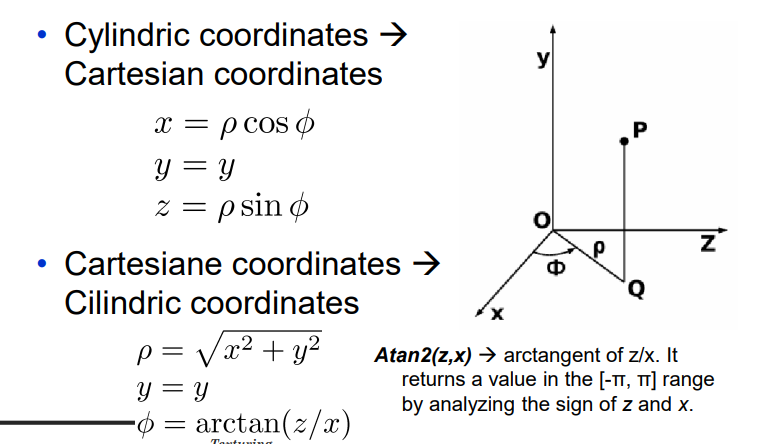
\includegraphics[width=0.5\textwidth]{images/project.png} 
    \caption{Cylindric Projection}
    \label{fig:immagine}
\end{figure}
\subsubsection{Enviroment mapping: Sphere mapping}
Mappatura dell'ambiente: una texture che rappresenta il colore dell'ambiente riflesso. Come coordinate UV può essere utilizzato il vettore di riflessione.
$ u= atan2(r_y,r_x) \\
 v= arccos(r_z)$ \\

Coordinate sferiche -> Coordinate cartesiane
$
x= \rho \ sin \theta \ cos \ \phi$ \\
\vspace{10pt} 
$y= \rho \ cos  \ \theta$ \\
$z=\rho \ sin\  \theta \ sin \ \phi$ \\
\vspace{10pt} 
Coordinate cartesiane  -> Coordinate sferiche 
$ \rho=\sqrt{x^2 + y^2+z^2}$
$ \phi=\arctan(z/x)$
$\theta=\arctan(\frac{y}{x^2+y^2+z^2})$

\subsubsection{Enviroment mapping: Cube mapping}
\begin{itemize}

\item Campionamento più uniforme della mappatura sferica.
\item È facile generare la mappa dell'ambiente.
\item Generazione delle coordinate uv a partire dal vettore di riflessione $ (r = (rx , ry , rz))$:
\begin{itemize}
    \item Il valore massimo definisce la faccia del cubo da utilizzare per la mappatura.
    \item Esempio: (-3.2 , 5.1 , -8.4) → faccia -Z
    \item Le coordinate sono ottenute dividendo il valore rimanente per il valore massimo (intervallo [-1,1]) e normalizzando i risultati tra [0,1].
    \item Esempio:$ (\left(-\frac{3.2}{8.4} , \frac{5.1}{8.4}\right) \rightarrow (-0.38, 0.61))$
    \item Per normalizzare i valori nell'intervallo [-1, 1] a [0, 1] aggiungiamo 1 e dividiamo per 2.
    \item Esempio: $(\left(\frac{(-0.38 + 1)}{2} , \frac{(0.61 + 1)}{2}\right) \rightarrow (0.31 , 0.80))$
\end{itemize}
\end{itemize}
\subsubsection{Texturing out of range}
\begin{figure}[H]
    \centering
    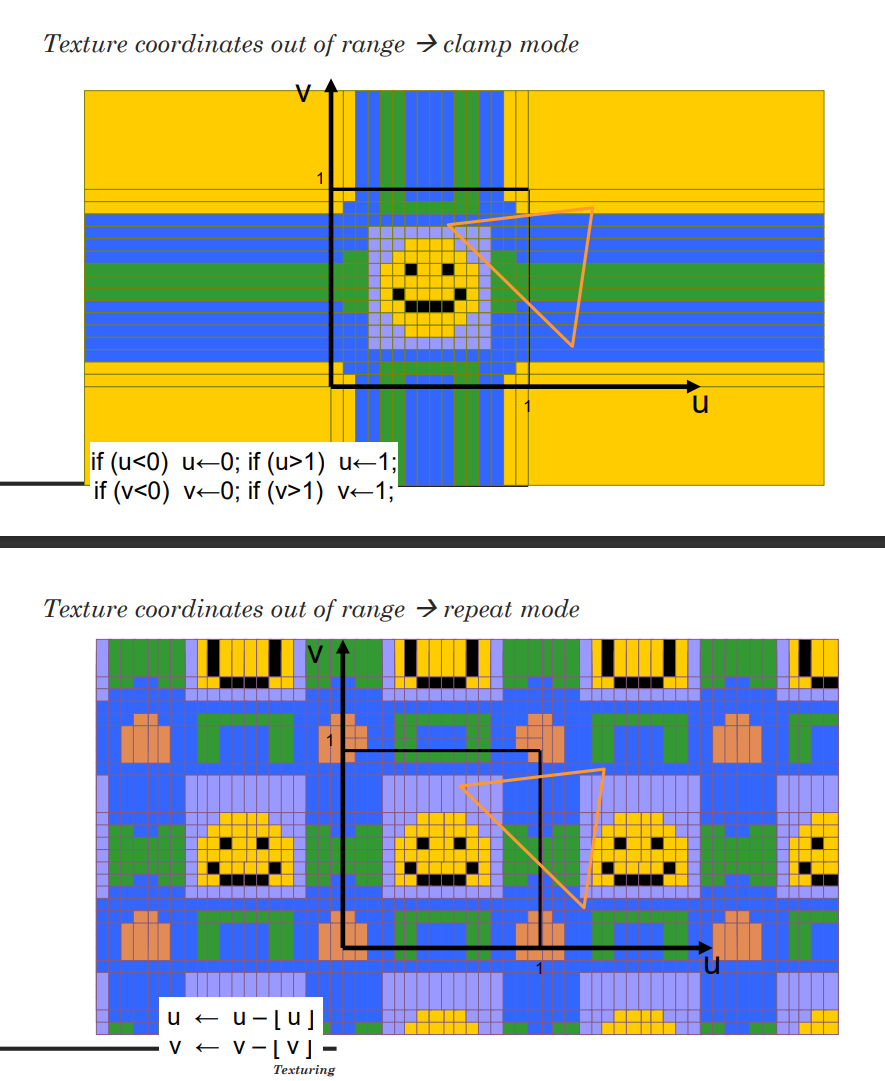
\includegraphics[width=0.5\textwidth]{images/TextOut.png} 
    \caption{Texture coordinates out of range}
    \label{fig:immagine}
\end{figure}
\subsection{Texture Look-Up}
\begin{figure}[H]
    \centering
    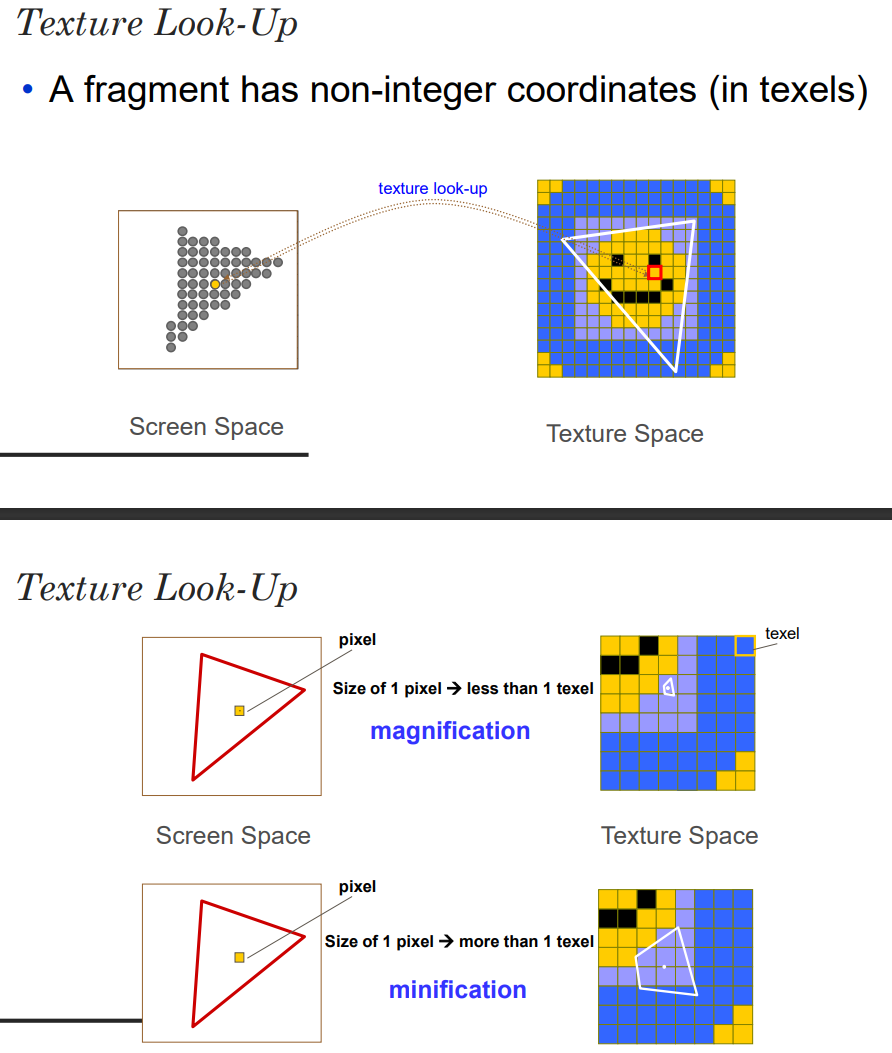
\includegraphics[width=0.5\textwidth]{images/lookup.png} 
    \caption{Texture Look-Up}
    \label{fig:immagine}
\end{figure}
\subsubsection{Maginification}
Due Soluzioni:
\begin{itemize}
    \item 
    Ottenere il texel quando cade
    (è equivalente a ottenere
    il texel più vicino)
    È equivalente a arrotondare le coordinate della texture al valore intero.
    \item Calcolare una media pesata dei quattro texel più vicini.
    Interpolazione bilineare
\end{itemize}
\begin{figure}[H]
    \centering
    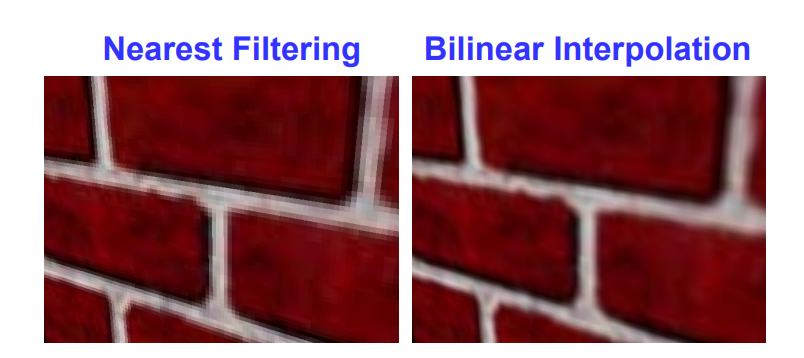
\includegraphics[width=0.5\textwidth]{images/magni.png} 
    \caption{Maginification}
    \label{fig:immagine}
\end{figure}
\subsubsection{Minification}
\subsubsection{Mip-Mapping}
Definiamo un fattore di scala $\rho = \text{texels/pixels}$ come il valore massimo tra $\rho_x$ e $\rho_y$, che può essere derivato dalla matrice di trasformazione geometrica e viene calcolato sui vertici, e interpolato per i frammenti. Il livello del mipmap è: $\log_2 \rho$, il livello 0 indica la massima risoluzione. Il livello non è necessariamente un numero intero, quindi deve essere arrotondato.
\begin{figure}[H]
    \centering
    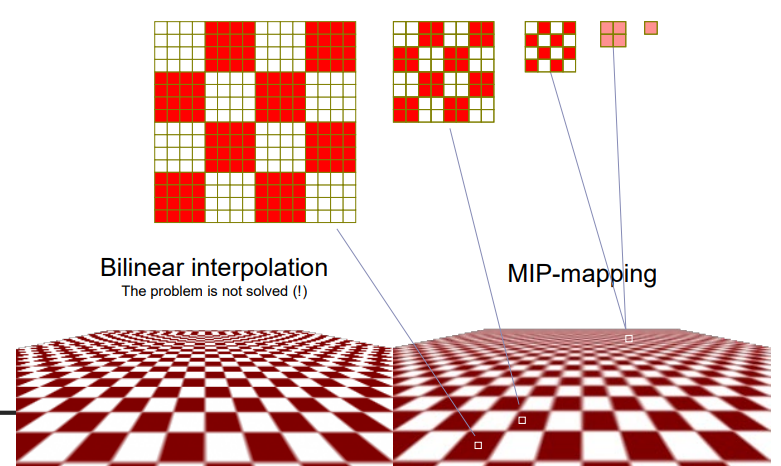
\includegraphics[width=0.5\textwidth]{images/MipMap.png} 
    \caption{Mip-Mapping \& Bilinear}
    \label{fig:immagine}
\end{figure}
\subsubsection{Bump Mapping}

L'aspetto di un oggetto può essere modificato utilizzando una tecnica chiamata \textit{Bump Mapping}.\\
$\vec{N_{new}}={\vec{N_{old}}}+\vec{D};$ \\
Il risultato è una perturbazione delle normali che altera il rendering senza modificare la geometria.\\
$\vec{D}=(\Delta x,\Delta y, \Delta z)$
\begin{figure}[H]
    \centering
    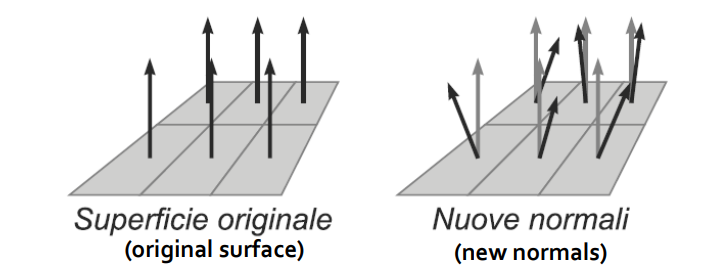
\includegraphics[width=0.5\textwidth]{images/Bump2.png} 
    \caption{Bump Mapping}
    \label{fig:immagine}
\end{figure}
\subsubsection{Displacement Mapping}
Utilizzando il displacement mapping, la geometria dell'oggetto 3D viene effettivamente modificata spostando i punti 3D della superficie:
$P_{new}=P_{old} + h*N $ \\
\begin{itemize}
    \item Il displacement mapping viene eseguito al momento del rendering e non modifica la geometria della scena.
    \item La differenza con il bump mapping è che la silhouette del modello 3D è correttamente deformata.
\end{itemize}
\begin{figure}[H]
    \centering
    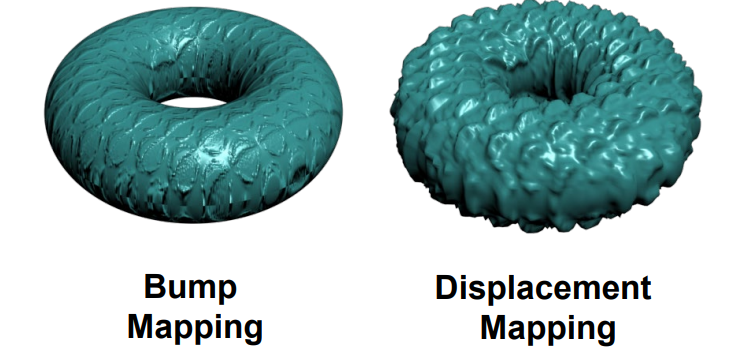
\includegraphics[width=0.5\textwidth]{images/BumpMap.png} 
    \caption{Bump Mapping \& displace Mapping}
    \label{fig:immagine}
\end{figure}